\chapter{Resultados}

%% Esto seria cierto si Q learning hubiera funcionado...
%%El problema de llevar inventario de un a\~no a otro se resolvi\'o f\'acilmente con el m\'etodo \textit{Q-learning}, pues su misma estructura requiere valores descontados de los estados futuros en cada estado presente. Para lograr el mismo efecto con el m\'etodo \textit{Policy Iteration}, ser\'ia necesario crear artificialmente d\'ias de entrenamiento antes y despu\'es del periodo de 365 d\'ias en el que los agentes est\'an aprendiendo, sin embargo, esto a\~nadir\'ia complejidad computacional.

En esta secci\'on se presentar\'a el c\'odigo utilizado para el modelo de aprendizaje reforzado, as\'i como los resultados en cada experimento realizado. El c\'odigo completo puede consultarse en el repositorio p\'ublico $https://github.com/fleoren/Tesis\_Maestria$. Para maximizar la reusabilidad y la posible exposici\'on a otras audiencias, tal c\'odigo est\'a escrito y documentado en ingl\'es.\\

Durante el aprendizaje se realizaron numerosos experimentos con diferentes metapar\'ametros (e.g. $\epsilon$ para el algoritmo $\epsilon-greedy$), par\'ametros del mundo (e.g. la penalizaci\'on por \'ordenes no cumplidas) y par\'ametros de los agentes (e.g. los m\'argenes de ganancia de cada uno). En esta secci\'on se presentar\'an algunos an\'alisis y resultados relevantes.\\

En general, el m\'etodo \textit{policy iteration} convergi\'o r\'apidamente, siendo capaz de encontrar estrategias \'optimas para todos los agentes en menos de 10 minutos. Asimismo, se encontr\'o que en la gran mayor\'ia de los casos (obtenidos con simulaciones), se obtiene un mejor desempe\~no para todo el sistema de cadena de suministro favoreciendo la estrategia inteligente sobre m\'etodos comunes, incluso si solamente uno de los agentes lo hace.

\section{C\'odigo: el Modelo, el Mundo y los Agentes}

A pesar de que nuestro sistema tiene seis roles, en realidad solamente cuatro de ellos toman decisiones:

\begin{itemize}
    \item El consumidor \textbf{obedece} a su necesidad interna de cerveza, mayor en fines de semana y festividades
    \item La tienda minorista \textbf{decide} cu\'anta cerveza va a comprar a la tienda de mayoreo
    \item La tienda de mayoreo \textbf{decide} cu\'anta cerveza va a comprar al almac\'en regional
    \item El almac\'en regional \textbf{decide} cu\'anta cerveza va a comprar a la f\'abrica
    \item La f\'abrica \textbf{decide} cu\'anta cebada va a comprar a los campos
    \item Los campos \textbf{obedecen} a sus ciclos de siembra y cosecha
\end{itemize}

A pesar de que, estrictamente, en nuestro sistema multiagente todos los roles son agentes, por claridad en la descripci\'on y el flujo del c\'odigo nos referiremos como agentes solamente a aquellos roles que toman decisiones. Las ecuaciones de los agentes en los extremos se pueden conectar f\'acilmente al sistema manteniendo la misma l\'ogica si suponemos que, para el consumidor, su \textit{policy} \'optimo es su demanda normal durante el a\~no, y para los campos, es su producci\'on.\\

Para construir todo el sistema, son necesarios varios elementos: los metapar\'ametros del modelo, los par\'ametros globales del mundo, los par\'ametros individuales de los agentes, los agentes como entidades funcionales, y las relaciones entre los agentes.\\

\subsection{El modelo: metapar\'ametros}

Existen cinco par\'ametros que son necesarios para asegurar el buen funcionamiento del modelo:

\begin{itemize}
    \item Semilla para realizaciones aleatorias, para permitir replicabilidad de experimentos, con valor permanente $20170130$
    \item Total de \'epocas (\textit{epochs}) de entrenamiento, es decir, cu\'antas iteraciones har\'a el modelo antes de llegar a un resultado final, con valor base $10,000$ pero flexible para diferentes experimentos
    \item Tiempo de comienzo, para que cada agente observe las cantidades demandadas por el agente inferior y calibre correctamente la magnitud de su propia demanda, con valor permanente $0.05\%$
    \item Epsilon ($\epsilon$), que controla la proporci\'on de explotaci\'on contra exploraci\'on y cuyo uso fue detallado en el cap\'itulo Aprendizaje Reforzado, con valor permanente $0.05\%$
    \item Lambda ($\lambda$), que controla el descuento de recompensas obtenidas en tiempos $t$ m\'as adelantados que el actual y cuyo uso fue detallado en el cap\'itulo Aprendizaje Reforzado, con valor permanente $90\%$
    \item Demanda m\'axima en un d\'ia para cualquier agente, para mantener las realizaciones dentro de un rango razonable, con valor permanente $75$, el cual es mucho mayor que la demanda diaria del consumidor (cuyo valor est\'a siempre por debajo de $4$ unidades)
\end{itemize}

\subsection{El mundo: par\'ametros globales}

El mundo contiene a los agentes, por lo tanto la mayor parte de los par\'ametros le pertenecen a estos. Sin embargo, el mundo necesita dos controles importantes para asegurar que el algoritmo aprende correctamente, los cuales podr\'ian definirse a nivel agente pero por simplicidad se mantendr\'an globales:

\begin{itemize}
    \item Costo por \'ordenes no cumplidas: valor base $2$, idealmente debe mantenerse debajo del margen m\'as peque\~no de los agentes para asegurar que es preferible vender cerveza que no hacer nada
    \item Costo de almacenamiento: valor base $10/365 = 0.027$; este debe ser mayor a cero para asegurar que los agentes no almacenan todo en el d\'ia $1$, suficientemente alto como para impactar en el margen si se almacena demasiado, pero suficientemente bajo como para que no sea redituable mantener cerveza almacenada m\'as de un a\~no
\end{itemize}

Por \'ultimo, dado que solamente se referir\'a como \textit{agentes} a aquellos que aprenden, se declaran las tendencias de demanda de consumidor y de oferta de los campos dentro de esta secci\'on. Estas tendencias se encuentran en dos archivos formato $.csv$ para permitir flexibilidad a cambios.

\subsection{Los agentes: funcionamiento e interrelaciones}

Cada uno de los agentes es creado como entidad funcional con el siguiente c\'odigo, ejemplificado para el agente de menudeo (\textit{retail}). La \'unica informaci\'on espec\'ifica que necesita cada agente es un nombre, su inventario inicial, sus precios de venta al agente inferior y compra al agente superior, y el costo de almacenamiento (el cual est\'a definido de manera global). Todos los dem\'as par\'ametros necesarios son establecidos al crear el mundo.

\begin{minted}{python}
retail_agent = Agent(name = "Retail", 
                    inventory = retail_ininv,
                    selling_price = retail_price,
                    buying_price = wholesale_price,
                    warehouse_price = warehouse_price)

\end{minted}

Cada agente es creado como una clase \textit{Agent} con varios m\'etodos que gobiernan la manera en que interact\'uan con el mundo y los otros agentes, como el proceso de compra/venta de cerveza a los agentes superiores e inferiores, y el pago recurrente por almacenamiento. Estos m\'etodos se ver\'an m\'as adelante, cuando se expongan las ecuaciones que los definen.\\

Una vez que los metapar\'ametros, los par\'ametros globales del mundo y los agentes han sido creados, el mundo se inicializa de la siguiente manera:

\begin{minted}{python}
# Creating Supply Chain Agents
customer_agent = Customer(customer_demand)
retail_agent = Agent(name = "Retail", 
                    inventory = retail_ininv,
                    selling_price = retail_price,
                    buying_price = wholesale_price,
                    warehouse_price = warehouse_price)
wholesale_agent = Agent("Wholesale", 
                    wholesale_ininv, 
                    wholesale_price,
                    regional_warehouse_price,
                    warehouse_price)
regional_warehouse_agent = Agent("Regional_Warehouse", 
                    regional_warehouse_ininv, 
                    regional_warehouse_price,
                    factory_price, 
                    warehouse_price)
factory_agent = Agent("Factory",
                    factory_ininv,
                    factory_price,
                    field_price,
                    warehouse_price)
fields_agent = Fields(fields_supply)

# Assigning interactions
retail_agent.downstream_agent = customer_agent
retail_agent.upstream_agent = wholesale_agent
wholesale_agent.downstream_agent = retail_agent
wholesale_agent.upstream_agent = regional_warehouse_agent
regional_warehouse_agent.downstream_agent = wholesale_agent
regional_warehouse_agent.upstream_agent = factory_agent
factory_agent.downstream_agent = regional_warehouse_agent
factory_agent.upstream_agent = fields_agent

\end{minted}

Como se puede notar, los ``agentes'' a los extremos de la cadena se inicializan de manera diferente. Dado que ambos obedecen estrategias fijas, en lugar de decidir y tener que aprender, el \'unico par\'ametro necesario es el comportamiento que deben obedecer.\\

Cada uno de los agentes que \textbf{deciden}, y por lo tanto pueden aprender, son inicializados con la misma clase \textit{Agent}, pero con sus par\'ametros de inventarios y precios propios. Por \'ultimo, se establecen las relaciones entre los agentes para crear la cadena. Esta manera de construir y definir expl\'icitamente los agentes y sus relaciones permite f\'acilmente a\~nadir o remover agentes de la cadena, si fuera necesario hacerla m\'as corta o larga.\\

Durante el aprendizaje, todos los agentes siguen el mismo conjunto de reglas (aprender cu\'anto tienen que comprarle al agente superior en cada d\'ia, maximizando la ganancia que obtienen de venderle al agente inferior, al tiempo de minimizar los costos de almacenamiento y la penalizaci\'on por \'ordenes no cumplidas), as\'i que las ecuaciones de ganancia y aprendizaje son las mismas. En este trabajo, se utilizar\'a la siguiente construcci\'on del mundo, con cierta notaci\'on para los distintos par\'ametros del mundo:

\begin{enumerate}
    \item Para cada agente \textit{$a$}, el agente superior en la cadena de suministro es \textit{$a+1$}; el inferior es \textit{$a-1$} y se representan con sub\'indices para cada atributo
    \item Cada agente tiene un precio de venta \textit{$p_{a}$}, un costo de almacenamiento \textit{$c_{a}$} y un costo por orden no cumplida (\textit{backlog}) \textit{$b_{a}$}
    \item En cada d\'ia \textit{$d$}, cada agente \textit{$a$} recibir\'a del agente superior \textit{$a+1$} la cantidad demandada por el primero en el d\'ia \textit{$d-1$}, sujeto a que tal cantidad sea menor o igual a la cantidad que el agente \textit{$a+1$} ten\'ia en el almac\'en
    \item En cada una de estas transacciones, cada agente recibe el dinero equivalente, basado en su respectivo precio de venta, e incurre en costos de almacenamiento y por \'ordenes no cumplidas
\end{enumerate}


Esto quiere decir que, independientemente del algoritmo de aprendizaje que usemos, cada agente \textit{a} calcula su ganancia en el d\'ia \textit{d} de la siguiente manera:

$$
ganancia_{a,d} = (p_{a} * ventas_{a, d}) 
$$
$$
\quad  \quad  \quad  \quad  \quad  \quad  \quad  \quad  \quad \quad  \quad   \quad  \quad - (b_{a}* (demanda_{a-1,d} - ventas_{a,d})) 
$$
$$
\quad  \quad  \quad  \quad  \quad  \quad  \quad  \quad - (p_{a+1}*ventas_{a+1, d-1})
$$
$$
\quad  \quad  \quad  \quad  \quad  \quad  \quad  \quad - (c_{a}*inventario_{a,d-1})
$$

Es decir, cada agente recibe el dinero correspondiente a las ventas que hace al agente inferior, paga el costo castigo relacionado a las \'ordenes no cumplidas, paga las \'ordenes hechas al agente superior y paga el costo de almacenamiento.\\

Dentro del m\'etodo existen tres funciones para lograr esta ecuaci\'on:

\begin{minted}{python}

def give_downstream(self, orders):
    # Checks if he has availability to fulfill order,
    # fulfills as much as he can
    if self.inventory >= orders:
        self.total_money = self.total_money + \
            (orders * self.selling_price)
        self.inventory = self.inventory - orders
        return orders
    else:
        orders_that_could_be_fulfilled = self.inventory
        # Sells all its inventory
        self.total_money = self.total_money + \
            (orders_that_could_be_fulfilled * self.selling_price)
        # If there were non fulfilled orders, those cause a penalty
        self.backlog = (orders - self.inventory) * backlog_cost
        self.total_money = self.total_money - self.backlog
        self.inventory = 0
        return orders_that_could_be_fulfilled

def receive_upstream(self, orders):
    # Receives orders from upstream agent first thing in the morning
    self.inventory = self.inventory + orders
    self.total_money = self.total_money - \
            (orders * self.buying_price)
     
def pay_for_warehousing(self):
        # Pays for warehousing of inventory: must be done either
        # "first thing in the morning" or "last time in the night"
        self.total_money = self.total_money - \
                (self.inventory * warehouse_price)
        self.total_warehousing_costs = self.total_warehousing_costs + \
                (self.inventory * warehouse_price)
                
\end{minted}

Cada uno de estos m\'etodos mapea limpiamente a los renglones: los primeros dos se refieren al precio propio y las ventas al agente inferior; el tercero se refiere al precio del agente superior y las ventas del agente superior (por lo tanto, las compras del agente de inter\'es); y por \'ultimo el cuarto es el costo de inventario y las cervezas guardadas.\\

Es importante notar que las reglas de funcionamiento del mundo lo convierten en un ambiente que, si bien no es estoc\'astico en el sentido estricto de la definici\'on, tampoco es puramente determinista: un agente que tome la misma acci\'on puede tener diferente recompensa de una realizaci\'on a otra debido a un manejo de inventario diferente del agente superior. El sistema  presenta un comportamiento m\'as estoc\'astico durante la fase de exploraci\'on, y tiende a uno completamente determinista durante la fase de explotaci\'on. Es por esto que en este trabajo, no se han incluido probabilidades de transici\'on (indicadas como $T(s, \pi(s), s'$ en las ecuaciones de secciones anteriores) en el modelo empleado, cada acci\'on tomada en un estado por un agente solo tiene una posible consecuencia, dada por las restricciones de inventario y los par\'ametros del mundo tales como costos y precios.\\

Si bien el c\'odigo del modelo fue construido para tener flexibilidad en los par\'ametros del mundo (como los precios de compra y venta de los agentes, o los costos de almacenamiento), la mayor parte de los resultados presentados en esta secci\'on fueron obtenidos con la misma combinaci\'on prudente de tales par\'ametros. Existen casos extremos, por ejemplo que todos los agentes comenzaran el a\~no con m\'as inventario del que necesitar\'an, y por lo tanto nunca necesitar\'an presentar una cantidad demandada ante sus respectivos agentes superiores. Otro caso extremo podr\'ia surgir si el costo de almacenamiento fuera mayor al margen de ganancia y que la penalizaci\'on por \'ordenes no cumplidas no compesara tal diferencia. En este trabajo no se explorar\'an estos casos extremos.\\

Una vez establecidas todas las relaciones entre todos los jugadores as\'i como los par\'ametros del mundo, se han obtenido dos formas diferentes de solucionar el juego: la primera con \textit{policy iteration} y la segunda con \textit{Q-learning}. En este trabajo no se ahondar\'a en los resultados de \textit{Q-learning} dado que el algoritmo no convergi\'o en un tiempo razonable, y tambi\'en dado que \textit{policy iteration}, a pesar de ser un algoritmo m\'as simple, dio buenos resultados en todas las simulaciones.

\section{Policy Iteration}

Las ecuaciones que describen el aprendizaje de un agente son:

\begin{enumerate}
    \item La ecuaci\'on de utilidad (recompensa) para cada agente $a$ en el d\'ia $d$:

$$
R(a, d) = r_{a,d} + \gamma*r_{a, d+1} + ... + \gamma^{364}*r_{a,d+364}
$$

    \item El vector de pol\'itica para cada agente tiene la siguiente forma, guardando en cada elemento la cantidad demandada al agente superior en cada tiempo $t$, que en este caso es cada d\'ia del a\~no:
    
$$
\pi(s) = \left \{ \pi(s)_{ t = 1}, \pi(s)_{ t = 22}, ..., \pi(s)_{ t = 365} \right \}
$$

\end{enumerate}

Se utilizan las ecuaciones planteadas en secciones anteriores para actualizar el vector de pol\'itica \'optima cuando se encuentra una nueva pol\'itica con un valor mayor.\\

El código utilizado para el aprendizaje con \textit{policy iteration} se encuentra a continuaci\'on. Los comentarios se han omitido, aunque los originales en ingl\'es pueden encontrarse en el repositorio de \textit{Github}, pues se ha procurado tener explicaciones en espa\~nol en el documento. Tambi\'en se omitieron las l\'ineas de c\'odigo que crean \textit{logs} o archivos utilizados para visualizaciones. \\

Antes de inicializar el aprendizaje, el par\'ametro $\epsilon$ juega su papel para crear la cantidad demandada cada d\'ia. Puede ser aleatoria (exploraci\'on) o la cantidad aprendida (explotaci\'on); dependiento de la realizaci\'on aleatoria del par\'ametro.

\begin{minted}{python}
def create_demand(day):
    x = np.random.uniform(0, 1)
    if x < p_exploration:  
        return np.random.randint(0,max_demand) 
    else: 
        return agent.best_policy[day-1]
\end{minted}

Una vez que se ha definido esa funci\'on, se utiliza un iterador para el total de \'epocas a entrenar, los agentes y los d\'ias del a\~no.

\begin{minted}[breaklines]{python}
for j in range(total_epochs):
    p_exploration = max(epsilon_greedy_converges_to ,(total_epochs - j) / total_epochs)
    day = 0
    for agent in agents:
        agent.inventory = agent.initial_inventory
        agent.total_warehousing_costs = 0
        agent.total_money = 0
        agent.backlog = 0

    while day < 365:  
        day+=1
        # Factory
        fulfilled_to_factory = min(factory_agent.current_policy[day-1],
                                   max(fields_agent.current_policy[day-1] - factory_agent.current_policy[day-1],0))
        factory_agent.receive_upstream(fulfilled_to_factory)
        factory_agent.current_policy[day-1] = fulfilled_to_factory
        # Regional Warehouse
        fulfilled_to_regional_warehouse = factory_agent.give_downstream(regional_warehouse_agent.current_policy[day-1])
        regional_warehouse_agent.receive_upstream(fulfilled_to_regional_warehouse)
        factory_agent.policy_inventory[day-1] = factory_agent.inventory
        regional_warehouse_agent.current_policy[day-1] = fulfilled_to_regional_warehouse
        # Wholesale
        fulfilled_to_wholesale = regional_warehouse_agent.give_downstream(wholesale_agent.current_policy[day-1])
        wholesale_agent.receive_upstream(fulfilled_to_wholesale)
        regional_warehouse_agent.policy_inventory[day-1] = regional_warehouse_agent.inventory
        wholesale_agent.current_policy[day-1] = fulfilled_to_wholesale
        # Retail
        fulfilled_to_retail = wholesale_agent.give_downstream(retail_agent.current_policy[day-1])
        retail_agent.receive_upstream(fulfilled_to_retail)
        wholesale_agent.policy_inventory[day-1] = wholesale_agent.inventory
        retail_agent.current_policy[day-1] = fulfilled_to_retail
        # Customer
        fulfilled_to_customer = retail_agent.give_downstream(customer_agent.current_policy[day-1])
        retail_agent.policy_inventory[day-1] = retail_agent.inventory

        for agent in agents:
            agent.current_payout[day-1] = agent.total_money
            if j == np.floor(total_epochs*agent.time_for_zero_policy):
                agent_demand = 0
            if j < warmstart_proportion * total_epochs:
                agent.average_downstream_demand = np.mean([agent.average_downstream_demand,
                                                           agent.downstream_agent.current_policy[day-1]])
                agent_demand = np.round(agent.average_downstream_demand)  
            else:
                agent_demand = create_demand(day)
            agent.current_policy[day-1] = agent_demand
            agent.pay_for_warehousing()
            if agent.current_payout[day-1] > agent.best_payout[day-1]:  
                agent.best_policy[day-1] = agent.current_policy[:][day-1]  
                agent.best_payout[day-1] = agent.current_payout[:][day-1]
                
\end{minted}

El iterador principal controla la cantidad de veces que se recorrer\'an los 365 d\'ias para cada agente, con el metapar\'ametro de \'epocas totales. En cada nuevo a\~no (cada nueva iteraci\'on) se reinicializan tanto el metapar\'ametro $\epsilon$ como los inventarios iniciales y el dinero de cada agente, mas no as\'i sus pol\'iticas aprendidas.\\

Cada a\~no (que tiene 365 d\'ias), cada agente ir\'a tomando decisiones diarias y monitoreando c\'omo afecta eso a su recompensa, la cual se estableci\'o como el dinero al final del experimento. As\'i, existen $4$ bloques de c\'odigo sumamente similares, solamente diferenciados por el nombre del agente que aprende. Por \'ultimo, hay dos l\'ineas adicionales para el ``agente'' consumidor: aunque \'el no aprende, es importante contabilizar correctamente las \'ordenes que le fueron cumplidas por el agente de menudeo.\\

El \'ultimo iterador en el c\'odigo, para cada agente, es donde sucede el aprendizaje. Primero, si todav\'ia se encuentra en el periodo de observaci\'on (controlado por un metapar\'ametro) asignar\'a como pol\'itica actual el promedio de la demanda observada de su agente inferior. En otro caso, monitorea si la acci\'on tomada el d\'ia anterior result\'o en una mejor recompensa en el d\'ia actual; si es el caso, reemplaza en el vector de pol\'itica \'optima; si no, conserva el vector \'optimo que tuviera anteriormente. De esta manera, acciones que resulten en mejores recompensas ir\'an construyendo la pol\'itica a seguir al final.\\

Es muy importante notar que todos los agentes son creados con el mismo m\'etodo \textit{Agent} y utilizan exactamente el mismo algoritmo para aprender, pero podr\'ian aprender \textit{policies} diferentes o ser impactados en menor o mayor medida por el efecto l\'atigo.\\

Cabe destacar que el vector de pol\'itica \'optima puede ser inicializado de cualquier manera. De manera razonable podr\'ia ser un vector de ceros, lo cual representa una estrategia de completa inacci\'on, un vector cuyos elementos son realizaciones de un generador de n\'umeros aleatorios para no imponer ninguna estrategia, etc. En este caso, se decidi\'o tener un periodo corto de observaci\'on al agente inferior, para tener una pol\'itica de l\'inea de base que podr\'ia juzgarse de sentido com\'un, y como presi\'on hacia una estrategia conservadora en contraste con una aleatoria. As\'i, todos los agentes inicializan su entrenamiento en un nivel relativamente estable alrededor del promedio de la demanda del agente inferior.\\

\subsection{Tiempo de entrenamiento}

Se hicieron pruebas con distintas iterationes totales y el tiempo que tomó realizarlas:

\begin{center}
\begin{tabular}{c|c}
Iteraciones     &  Tiempo\\
1,000     &  25 seg\\
10,000     &  4 min\\
100,000     &  40 min\\
1,000,000     & 6.5 h
\end{tabular}
\end{center}

Se puede notar que el tiempo necesario para iteraciones crece de forma lineal, pues los agentes no deben aumentar la cantidad de informaci\'on que aprenden a medida que el tiempo pasa. Incluso si se decidiera tomar la opci\'on de $1,000,000$ de iteraciones, el modelo entrena suficientemente r\'apido como para reentrenarlo diario de ser necesario (ante cambios abruptos en demanda u oferta).

\subsection{Mundo ideal: agentes inteligentes}

Los agentes aprenden estrategias que siguen el comportamiento de la oferta, lo cual es el comportamiento esperado dado que en las especificaciones iniciales, se defini\'o manualmente que la demanda anual no sobrepasara la oferta anual. Este resultado puede observarse en las figuras \ref{politer_payouts_1000} a \ref{politer_payouts_1000000}, en donde se presentan las pol\'iticas encontradas con $1k$, $10k$, $100k$ y $1M$ iteraciones. \\

\begin{figure}[!htb]
   \begin{minipage}{0.48\textwidth}
     \centering
     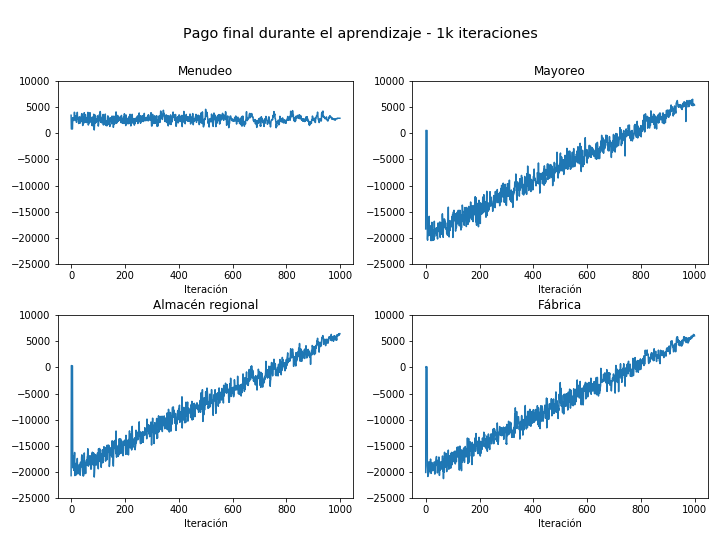
\includegraphics[width=1\linewidth]{tesis_tex/figs/policyiteration_payouts_1000.png}
     \caption{Evoluci\'on de recompensas con 1k iteraciones}\label{politer_payouts_1000}
   \end{minipage}\hfill
   \begin{minipage}{0.48\textwidth}
     \centering
     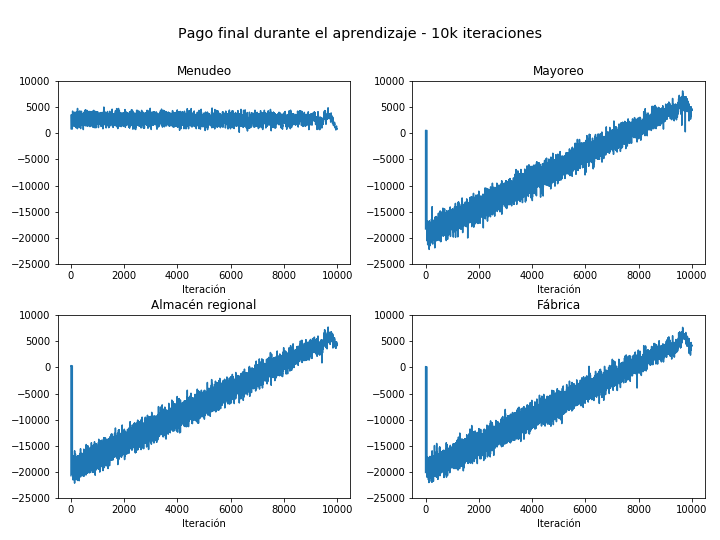
\includegraphics[width=1\linewidth]{tesis_tex/figs/policyiteration_payouts_10000.png}
     \caption{10k iteraciones}\label{politer_payouts_10000}
   \end{minipage}
\end{figure}

\begin{figure}[!htb]
   \begin{minipage}{0.48\textwidth}
     \centering
     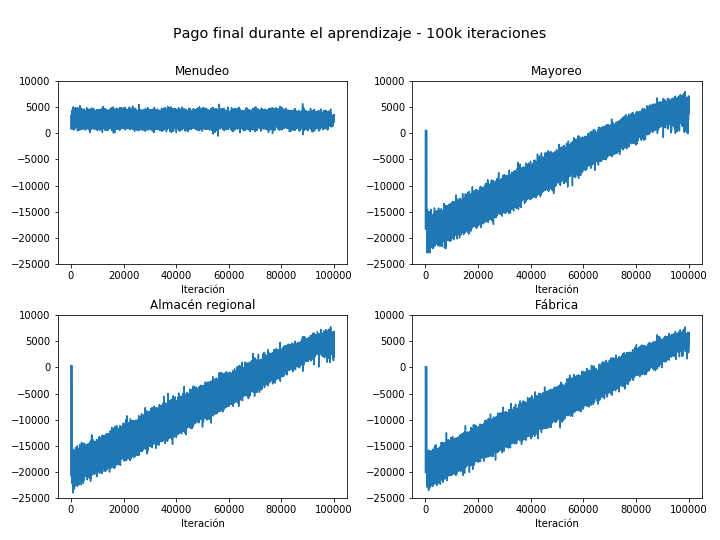
\includegraphics[width=1\linewidth]{tesis_tex/figs/policyiteration_payouts_100000.png}
     \caption{100k iteraciones}\label{politer_payouts_100000}
   \end{minipage}\hfill
   \begin{minipage}{0.48\textwidth}
     \centering
     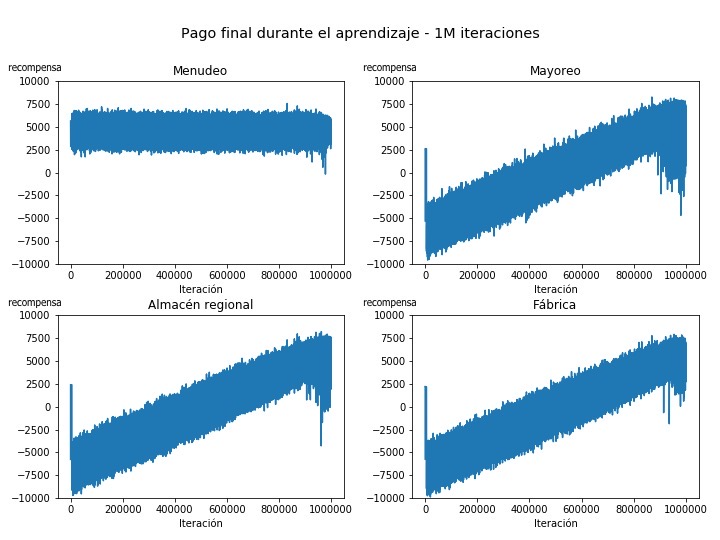
\includegraphics[width=1\linewidth]{tesis_tex/figs/policyiteration_payouts_1000000.png}
     \caption{1M iteraciones}\label{politer_payouts_1000000}
   \end{minipage}
\end{figure}

Es esperado observar  que todos los agentes presentan una tendencia positiva al encontrar mejores \textit{policies} en cada iteraci\'on del algoritmo. Sin embargo, es interesante notar que la funci\'on de valor del agente Menudeo empieza (despu\'es de un periodo de pre-calentamiento de $0.5\%$ del total de iteraciones) en un punto mucho m\'as cercano al \'optimo que los otros agentes. Esto puede explicarse porque, dada la configuraci\'on del mundo, el agente Menudeo tiene informaci\'on directa de la demanda del consumidor, y por lo tanto puede ajustar su pol\'itica mucho m\'as r\'apidamente.\\

El algoritmo converge de manera relativamente r\'apida: en las figuras  \ref{politer_payouts_1000} a \ref{politer_payouts_1000000} se puede observar que, con diferente n\'umero de iteraciones, el comportamiento del crecimiento de la funci\'on de valor (inferida de la pol\'itica \'optima en la iteraci\'on $i$) es similar. Asimismo, en las figuras \ref{politer_policies_1000} a \ref{politer_policies_1000000} se puede observar una comparaci\'on de las pol\'iticas obtenidas con los mismos umbrales de iteraciones: la forma es extremadamente parecida sin importar la cantidad de iteraciones. Este fen\'omeno nos indica que no es necesario un n\'umero alto de iteraciones, pues se encuentra el valor m\'aximo y la forma correcta de la pol\'itica \'optima con solamente $10,000$ iteraciones. Con las condiciones de \textit{hardware} y \textit{software} especificadas en secciones anteriores, este proceso tarda un poco menos de 5 minutos.\\

Otra manera de analizar la r\'apida convergencia al \'optimo del algoritmo es comparando las recompensas finales (asociadas a la estrategia \'optima encontrada) para cada agente, con diferente n\'umero de iteraciones. En la figura \ref{money_over_time} se puede observar que no es necesario un n\'umero alto de iteraciones, ya que el resultado final es sumamente estable.\\

\begin{figure}[H]
\caption{Comparaci\'on de recompensa final con diferente total de iteraciones}
\label{money_over_time}
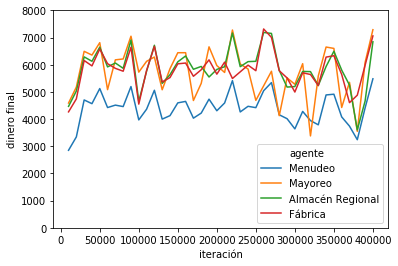
\includegraphics[width=10cm]{tesis_tex/figs/evaluating_interations_money.png}
\centering
\end{figure}

Las pol\'iticas aprendidas tienen el comportamiento esperado: todos los agentes compran cantidades altas durante ambos picos de producci\'on en verano, con la finalidad de abastecerse lo m\'as posible para las ventas del resto del a\~no. Es importante recordar que estas pol\'iticas \'optimas dependen de la selecci\'on de par\'ametros del mundo (precios, costos, etc.) en gran medida, as\'i como los metapar\'ametros (tiempo de calentamiento, $\epsilon$, etc.), lo que implica que es necesario realizar un entrenamiento nuevo en caso de que estos cambien, o si de un a\~no a otro los agentes tienen, por ejemplo, diferentes inventarios iniciales. Este problema puede ser resuelto entrenando un modelo como \textit{Q-learning}, opci\'on que se explorar\'a de manera superficial m\'as adelante en esta secci\'on.\\

\begin{figure}[!htb]
   \begin{minipage}{0.48\textwidth}
     \centering
     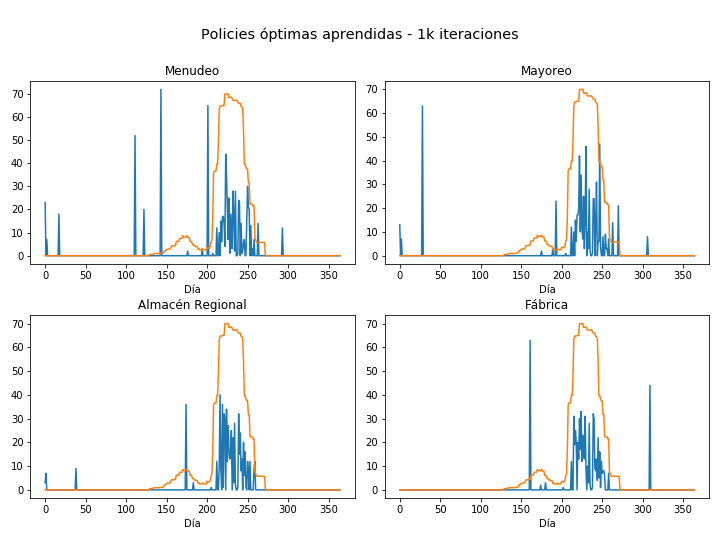
\includegraphics[width=1\linewidth]{tesis_tex/figs/policyiteration_policies_1000.png}
     \caption{Evoluci\'on de recompensas con 1k iteraciones}\label{politer_policies_1000}
   \end{minipage}\hfill
   \begin{minipage}{0.48\textwidth}
     \centering
     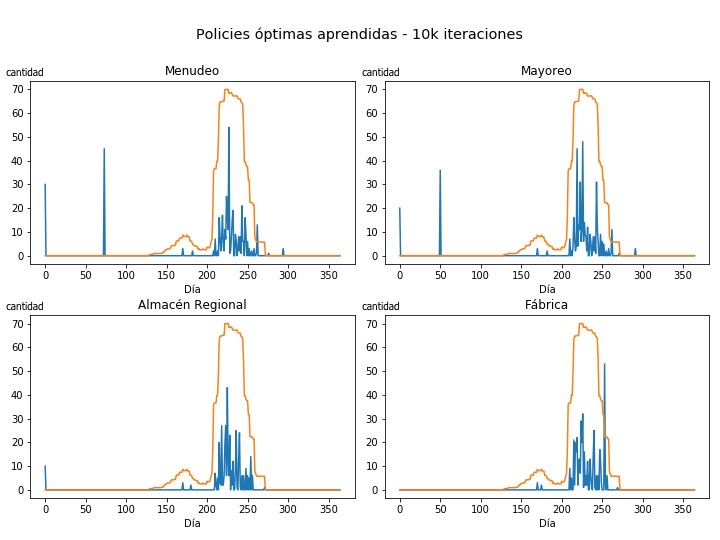
\includegraphics[width=1\linewidth]{tesis_tex/figs/policyiteration_policies_10000.png}
     \caption{10k iteraciones}\label{politer_policies_10000}
   \end{minipage}
\end{figure}

\begin{figure}[!htb]
   \begin{minipage}{0.48\textwidth}
     \centering
     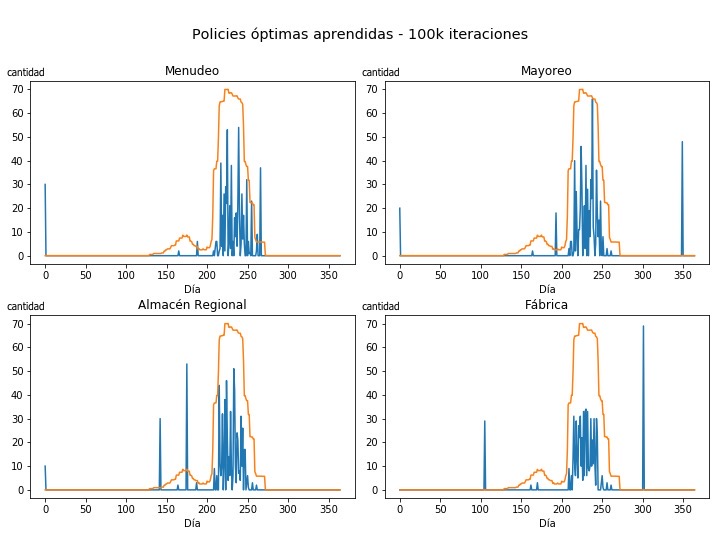
\includegraphics[width=1\linewidth]{tesis_tex/figs/policyiteration_policies_100000.png}
     \caption{100k iteraciones}\label{politer_policies_100000}
   \end{minipage}\hfill
   \begin{minipage}{0.48\textwidth}
     \centering
     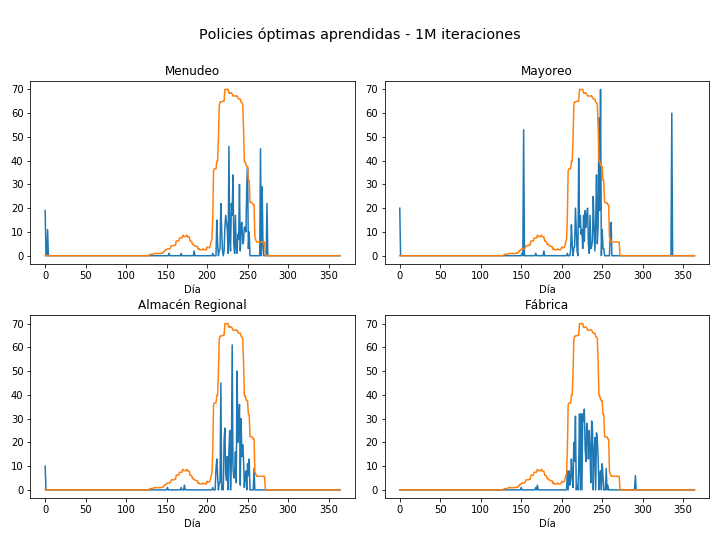
\includegraphics[width=1\linewidth]{tesis_tex/figs/policyiteration_policies_1000000.png}
     \caption{1M iteraciones}\label{politer_policies_1000000}
   \end{minipage}
\end{figure}

Durante el an\'alisis de las pol\'iticas y sus resultados, sali\'o a la luz un fen\'omeno no esperado que afecta de manera distinta a los agentes, tal que en algunas iteraciones resultan con recompensas m\'as bajas de lo esperado. Para profundizar en esto, se explor\'o la posibilidad de que no todos los agentes tomen decisiones \'optimas, cuyos resultados son presentados en el siguiente apartado. \\

\subsection{Agentes con diferentes niveles de aprendizaje}

Se ha hablado ya de las estrategias \'optimas obtenidas por el algoritmo de \textit{policy iteration}, sin embargo es de suma importancia comparar el potencial beneficio que podr\'ian tener los agentes tomando como l\'inea base una estrategia cre\'ible pero poco optimizada. Se busca responder a preguntas como: ¿vale la pena construir, entrenar y seguir el modelo, comparado con una estrategia de sentido com\'un?, o ¿es preferible usar la estrategia encontrada por el modelo, incluso si los dem\'as agentes en la cadena toman otro acercamiento?\\

 Para explorar estos escenarios, se definen dos tipos de estrategias y varias combinaciones de ellas. La primera estrategia, relativamente b\'asica, es una que dictar\'ia el sentido com\'un: cada agente calcula el promedio de peticiones del agente inferior durante los \'ultimos 5 d\'ias, y fija ese n\'umero como su demanda al agente superior. Por otro lado, la segunda estrategia, \'optima seg\'un el resultado del algoritmo \textit{policy iteration}, responde tanto a un periodo m\'as largo, como a factores adicionales tales como el costo de oportunidad de perder una orden comparado con el costo de almacenamiento. En el mundo ideal, que se explor\'o en la secci\'on anterior, todos los agentes siguen la estrategia encontrada por el modelo. Sin embargo, es posible que una situaci\'on m\'as realista contenga una mezcla de estrategias para cada agente, dado que cada uno es independiente y puede tomar sus propias decisiones. Existen varios escenarios intermedios entre el mundo ideal y el mundo en el que todos los agentes siguen la estrategia b\'asica; en esta secci\'on se explorar\'an los resultados si:\\
 
 \begin{enumerate}
     \item Todos los agentes siguen la estrategia b\'asica (el cual se tomar\'a como escenario base)
     \item Un agente, que no es el analizado, sigue la estrategia aprendida, y todos los dem\'as (incluyendo al de inter\'es), siguen la b\'asica
     \item Un agente, que es el analizado, sigue la estrategia aprendida, y todos los dem\'as siguen la b\'asica
     \item Todos los agentes siguen la estrategia aprendida
 \end{enumerate}

Para este an\'alisis, se cre\'o un \'indice que se puede interpretar como la ganancia en porcentaje con respecto a la estrategia base, es decir, un valor del \'indice de $0.5\%$ significa que esa estrategia report\'o $50\%$ m\'as dinero al final de ese a\~no para ese agente que si hubiera tomado la estrategia b\'asica. Cualquier valor positivo del \'indice, entonces, implica un desempe\~no mejor que la l\'inea base, un valor negativo significa un desempe\~no peor.\\

Tambi\'en es relevante explorar si la estrategia \'optima es preferible en cualquier escenario respecto a los par\'ametros del mundo (inventarios iniciales, precios de compra/venta, costo de almacenamiento, entre otros). Para analizar este aspecto simult\'aneamente, en cada nueva iteraci\'on se reinicializan todos los valores de tales par\'ametros de manera casi aleatoria; con restricciones de valores no-negativos para todos, y adicionalmente para los m\'argenes de los agentes. As\'i, el an\'alisis abarca una gran cantidad de casos y demuestra flexibilidad ante condiciones iniciales.\\

En la figura \ref{ev_policies_dumb} se puede ver una comparaci\'on del desempe\~no de todos los agentes con respecto a la l\'inea base elegida. Se muestra la l\'inea base, o la estrategia \textit{nadie \'optima} como una l\'inea azul punteada. Las dos curvas de comparaci\'on son: una combinaci\'on de estrategias en las que solamente el agente indicado toma y actualiza sus decisiones con el algoritmo de aprendizaje \textit{un agente \'optimo} y una combinaci\'on en la que todos los agentes aprenden con el algoritmo. Para esta figura se hicieron $250$ realizaciones del algoritmo con $1000$ etapas de aprendizaje, inicializando todos los par\'ametros del mundo de manera aleatoria cada vez, con restricciones m\'inimas relacionadas a los rangos de cada variable (por ejemplo, asegurar m\'argenes e inventarios no negativos)\\

En general, las distribuciones de índices relacionados a todos los agentes usando las estrategias \'optimas (obtenidas del algoritmo de aprendizaje), se encuentran a la derecha de las distribuciones de un solo agente aprendiendo. Esto es el comportamiento esperado, pues uno de los principales castigos para todos los agentes es el costo por orden no cumplida, y si no aprenden que deben tener suficiente inventario para cubrir esas \'ordenes, siempre cargar\'an con ese tipo de costos. Queda claro que es preferible para todos los agentes en conjunto trabajar de manera \'optima (con aprendizaje) al mismo tiempo, sin importar los par\'ametros iniciales de costos, inventarios o m\'argenes. Esta comparaci\'on puede consultarse de manera m\'as puntual en el siguiente par de tablas, para la cual es importante recordar que el cero es la l\'inea base, as\'i que un comportamiento positivo significa un resultado por encima de ella.\\

\hspace{5pt}

\begin{tabular}{ |p{3cm}||p{1.7cm}|p{1.9cm}|p{2.3cm}|p{1.7cm}|  }
 \hline
 \multicolumn{5}{c}{Valor esperado de los \'indices de cada estrategia} \\
 \hline
 Agente & Nadie & Solo otro & Solo \'el mismo & Todos\\
 \hline
 Menudeo & 0 & 1.60 & 1.18 & 2.54\\
 Mayoreo & 0 & -0.22 & 0.27 & 2.47\\
 Almac\'en regional & 0 & -0.23 & 0.13 & 2.76\\
 F\'abrica & 0 & 1.68 & 1.01 & 2.54\\
 \hline
\end{tabular}


\hspace{5pt}

\begin{tabular}{ |p{3cm}||p{1.7cm}|p{1.9cm}|p{2.3cm}|p{1.7cm}|  }
 \hline
 \multicolumn{5}{c}{Desviaci\'on est\'andar de los \'indices de cada estrategia} \\
 \hline
 Agente & Nadie & Solo otro & Solo \'el mismo & Todos\\
 \hline
 Menudeo & 0 & 0.84 & 0.85 & 0.97\\
 Mayoreo & 0 & 1.43 & 1.38 & 1.01\\
 Almac\'en regional & 0 & 1.38 & 1.60 & 1.13\\
 F\'abrica & 0 & 0.94 & 0.68 & 0.97\\
 \hline
\end{tabular}

\hspace{25pt}

Es importante notar que las distribuciones de \'indices cuando solamente un agente utiliza la estrategia de aprendizaje se encuentran constantemente a la derecha de la l\'inea base. Esto quiere decir que siempre es preferible utilizar la estrategia de aprendizaje, sin importar la estrategia que el resto de los agentes escojan.\\

Una situaci\'on muy interesante se presenta en el escenario complementario al anterior: se ha establecido que es preferible usar la estrategia aprendida a pesar de que los otros agentes no hagan lo mismo, pero ¿qu\'e pasa con los agentes que no escogen la estrategia aprendida, cuando otro agente s\'i lo hace? El comportamiento esperado ser\'ia que la utilidad fuera mejor que si nadie estuviera aprendiendo, dado que al menos uno de los agentes estar\'ia optimizando su inventario. Sin embargo, esto no es cierto para todos los agentes: tanto \textit{mayoreo} como \textit{almac\'en regional} tienen valor esperado negativo si solamente otro agente toma acciones inteligentes y cada uno de ellos sigue la estrategia base. Adem\'as, las desviaciones est\'andar asociada a estas distribuciones - y, en realidad, a las de todos los escenarios - son considerablemente mayores a las correspondientes a los otros dos agentes. Esto quiere decir que los agentes hacia el centro de la cadena tienen mayor presi\'on de seguir estrategias inteligentes, independientemente de si los dem\'as agentes en la cadena lo hacen. Este comportamiento se puede ver tambi\'en en la figura \ref{ev_policies_dumb}.\\

Por \'ultimo, podemos observar que las distribuciones de un solo agente tomando decisiones \'optimas son diferentes a pares: las de menudeo y f\'abrica son similares entre s\'i, al igual que las de mayoreo y almac\'en regional. Es notable que este comportamiento se presenta en los dos agentes que tienen una realidad diferente, ligada a agentes con estrategias estables y de donde provienen la demanda y oferta reales. El agente de menudeo siempre podr\'a vender todo su inventario lo m\'as pronto posible, dado que el comprador siempre tiene demanda positiva. Por otro lado, el agente de f\'abrica tambi\'en carga con presi\'on de los agentes inferiores de reducir sus costos de \'ordenes no cumplidas, as\'i que tambi\'en tiene asegurado vender su inventario pronto, mientras no compre cantidades innecesariamente altas. Los agentes de mayoreo y almac\'en regional no tienen ninguna de estas consideraciones.\\

Una posible hip\'otesis para este comportamiento se remonta al efecto l\'atigo: aquellos agentes m\'as cercanos a la informaci\'on pueden reaccionar m\'as r\'apidamente a cambios y tomar decisiones m'as ego\'istas que aquellos en medio de la cadena de suministro. As\'i, el agente menudeo tiene cercan\'ia al consumidor y el agente f\'abrica tiene cercan\'ia a los campos y conocen directamente ciertas partes de la informaci\'on del sistema, lo cual les permite tener estrategias m\'as s\'olidas y menos dependientes de lo que decidan los dem\'as agentes.\\

En conclusi\'on, para cualquier agente es preferible usar la estrategia aprendida, sin importar lo que hagan los dem\'as agentes. Adem\'as, los agentes en los extremos de la cadena sufren menor presi\'on por varianza en la informaci\'on recibida directamente del consumidor y de los campos.\\

\begin{figure}[H]
\caption{Comparaci\'on de desempe\~no entre combinaciones de estrategias}
\label{ev_policies_dumb}
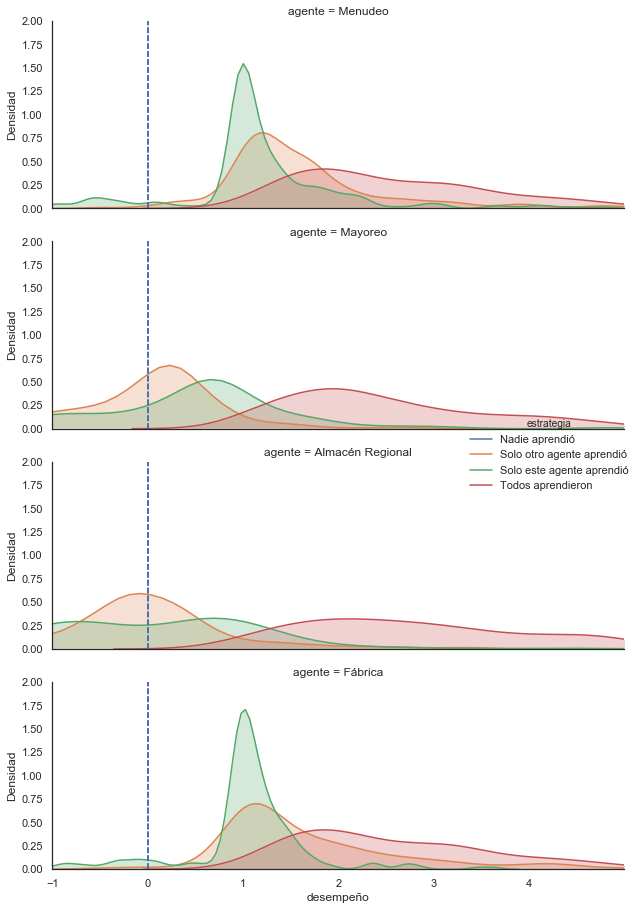
\includegraphics[width=9cm]{tesis_tex/figs/evaluating_policies_dumb_to_smart.png}
\centering
\end{figure}

\section{Q-Learning}

Este m\'etodo encuentra, para cada estado, la acci\'on que acercar\'a al agente lo m\'as posible al \'optimo. Idealmente, la pol\'itica \'optima es equivalente con cualquiera de ambos m\'etodos. \textit{Q-learning} permite m\'as libertad respecto a empezar a jugar el juego a mitad de a\~no, arreglar malas decisiones tomadas por los agentes en periodos anteriores gracias a su adaptabilidad ante cambios estoc'asticos, etc. Sin embargo, al tener que explorar estados a los cuales los agentes llegan despu\'es de haber tomado estrategias que no son \'optimas, es un algoritmo mucho m\'as pesado computacionalmente.\\

Las ecuaciones que describen el aprendizaje de un agente son:

\begin{enumerate}
    \item La ecuaci\'on de utilidad (o recompensa) para cada agente $a$ en el d\'ia $d$:

$$
R(a, d) = r(a,d) + \gamma*r_{a, d+1} + ... + \gamma^{364}*r_{a,d+364}
$$

Donde la recompensa del agente \textit{a} en el d\'ia \textit{d} es la ganancia relacionada a sus respectivas transacciones, como se defini\'o al principio de este cap\'itulo. Es importante notar la importancia de tomar un periodo de un a\~no despu\'es del d\'ia $d$ sin importar en qu\'e d\'ia espec\'ifico se encuentre el agente: de esta manera, el agente aprender\'a si tiene que llegar al d\'ia $365$ con inventario en almacenes.\\

El c\'odigo que describe esta ecuaci\'on es:

\begin{minted}[breaklines]{python}
lambdas = [(lambda_q_learning**n) for n in range(365)]
agent.q_function_reward_for_action[day-1] = agent.current_payout[day-1] - agent.current_payout[day-2]
rewards = agent.q_function_reward_for_action[day-1:] + agent.q_function_reward_for_action[0:day-1]
discounted_rewards = np.multiply(rewards, lambdas)
r_s_a = np.sum(discounted_rewards)
\end{minted}


\item La funci\'on Q para cada agente $a$ dado su estado, el d\'ia $d$ con cierto inventario $inv$:

$$
Q_{a}(inv_{d},compra_{d}) = r_{a, (d, inv, compra)} + \gamma * \max_{compras}{Q_{a}(inv_{d} + compra_{d}, compras_{d+1}}
$$

El c\'odigo que describe la actualizaci\'on de la funci\'on $Q$ en cada paso es el siguiente. De manera similar que para \textit{policy iteration}, se itera por agente. Para cada uno de ellos, primero se identifica cu\'al es el siguiente estado (d\'ia $+1$, inventario al final del d\'ia). Despu\'es se busca en la tabla que guarda todos los aprendizajes pasados; si se encuentra el escenario, se maximizan todas las posibles recompensas encontradas y se asigna el valor a $Q$ con aquella que optimice; si no, se asigna el valor $0$ a la funci\'on $Q$. 

\begin{minted}[breaklines]{python}
subset_s_prime_a_all = q_learning_df.loc[(q_learning_df['agent'] == (agent.name)) & (q_learning_df['day'] == (next_day)) & (q_learning_df['inventory'] == (agent_inventory + agent_demand))]

if subset_s_prime_a_all.shape[0] > 0:
    max_q_s_prime_a_all = subset_s_prime_a_all['q_s_a'].max()
else:
    max_q_s_prime_a_all = 0

q_s_a = r_s_a + (lambda_q_learning * max_q_s_prime_a_all)
\end{minted}

Para cada agente, su estado es un vector de longitud $2$: en el d\'ia $d$ es el inventario que tiene en el almac\'en, y las acciones que puede tomar en cada estado se representan como un vector de longitud $1$: son las diferentes cantidades que puede comprarle al agente superior.
\end{enumerate}

Adem\'as, similarmente a \textit{policy iteration}, se implement\'o este algoritmo en la modalidad \textit{greedy}, con $\epsilon$ empezando en $1.00$ y terminando en $0.05$.

\subsection{Tiempo de entrenamiento}

El resultado de \textit{Q-learning} es fundamentalmente diferente que el de \textit{policy iteration}. El \'ultimo solamente itera en cuatro vectores de longitud 365 (dado que hay 4 agentes, y 365 d\'ias en un a\~no), manteniendo para cada agente solamente uno en la memoria de largo plazo: aquel que se ha determinado como el \'optimo hist\'orico. Por otro lado, el primero explora estados del mundo, incluso si no provienen de acciones ``buenas'' y mantiene en la memoria de largo plazo la mejor acci\'on a tomar si se llega a ese estado, adem\'as del valor de la funci\'on $Q$ para cada una de las posibles acciones exploradas. Esto significa que en cada iteraci\'on, el conocimiento de cada agente aumenta, pues recuerda la mejor acci\'on a tomar para cada estado, el cual es una combinaci\'on del d\'ia del a\~no y el inventario en tal d\'ia.\\

A diferencia de las iteraciones de \textit{policy iteration}, las iteraciones de \textit{Q-learning} toman m\'as memoria, y por lo tanto m\'as tiempo, a medida que el modelo va entrenando. En la figura \ref{q_learning_times} puede observarse este comportamiento, el cual se ajusta a un modelo polinomial $y=3.59x^{0.452}$ con una $R^2=0.975$. Esto quiere decir que crece m\'as lento que un modelo lineal, sin embargo la tasa es suficientemente grande como para convertirlo en un modelo prohibitivo desde el punto de vista de tiempo necesario para entrenamiento.

\begin{figure}[H]
\caption{Tiempo (segundos) por iteraci\'on en Q-learning}
\label{q_learning_times}
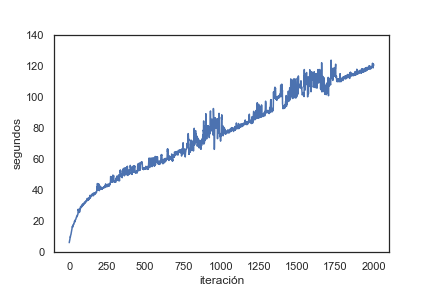
\includegraphics[width=9cm]{tesis_tex/figs/q_learning_times.png}
\centering
\end{figure}

Al notar el comportamiento creciente del tiempo por iteraci\'on, se hicieron varias pruebas para documentar el tiempo necesario para correr el algoritmo de aprendizaje. En secciones anteriores se mostr\'o que $10,000$ iteraciones eran suficientes para que \textit{policy iteration} encontrara \textit{policies} \'optimas en menos de $10$ minutos; sin embargo, para obtener $10,000$ iteraciones en \textit{Q-learning}, parecen necesarias m\'as de 3 semanas de entrenamiento continuo. Adem\'as, dado que por definici\'on, este \'ultimo explora y aprende a reaccionar a estados a\'un si no son \'optimos, es probable que $10,000$ iteraciones no sean suficientes para tener un resultado utilizable.

\begin{center}
\begin{tabular}{c|c}
Iteraciones     &  Tiempo\\
1,000     &  15 horas\\
2,000     &  47 horas\\
10,000     & 25 d\'ias (est)
\end{tabular}
\end{center}

\subsection{Estrategias}

Como se ha descrito anteriormente, los resultados de \textit{Q-learning} tienen una forma muy extensa: para cada agente, existe un conjunto de posibles acciones en cada estado (combinaci\'on de d\'ia e inventario) y sus respectivos valores de la \textit{funci\'on Q}. La manera de obtener la acci\'on \'optima para cada agente en cada tiempo $t$ es por medio de la b\'usqueda de la acci\'on $a$ que maximiza la \textit{funci\'on Q} dado el estado $s$, es decir dado el inventario. En la figura \ref{q_learning_results} se puede visualizar esta estructura.\

\begin{figure}[H]
\caption{Estructura de resultados de Q-learning}
\label{q_learning_results}
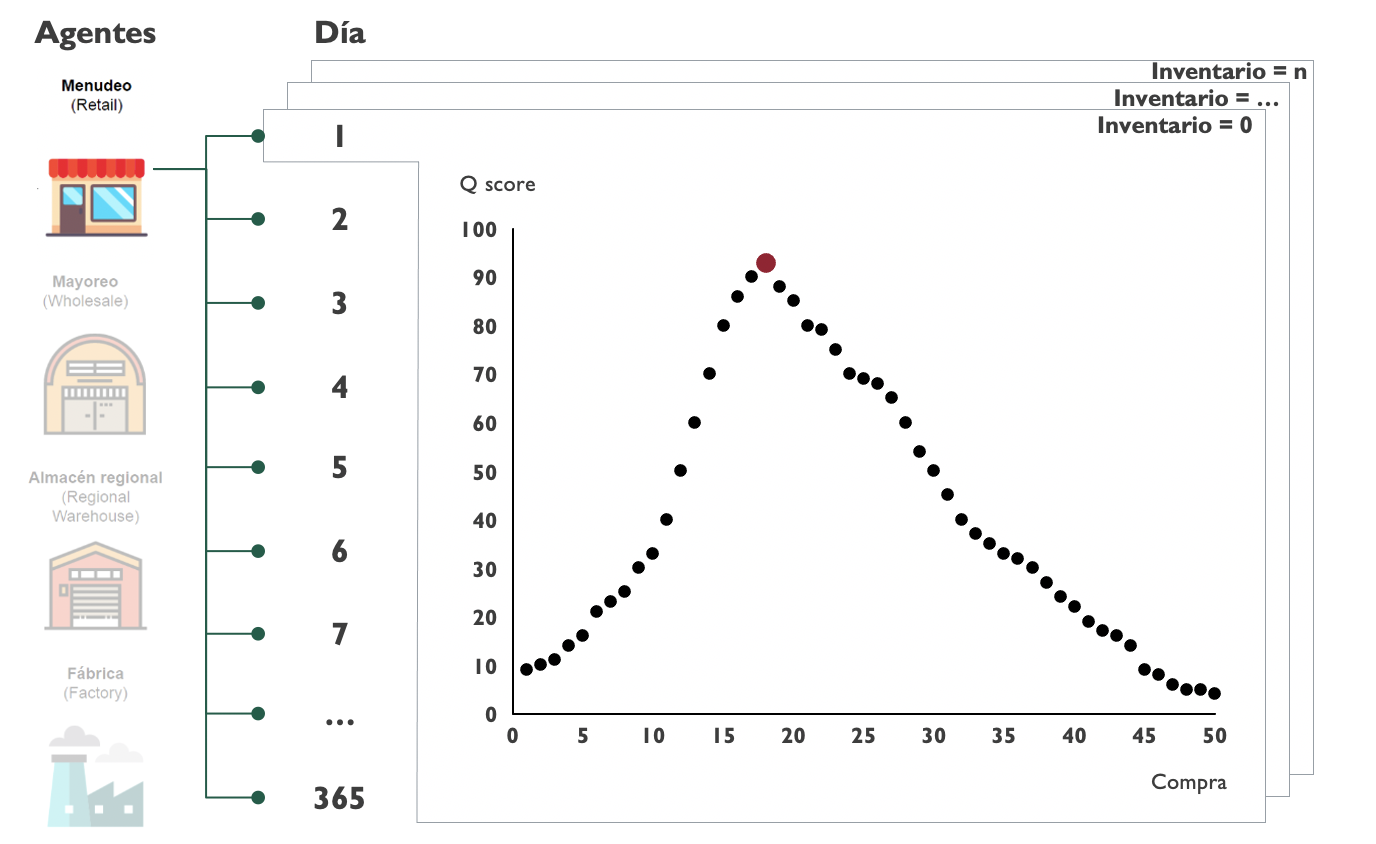
\includegraphics[width=12cm]{tesis_tex/figs/q_learning_results.png}
\centering
\end{figure}

En sentido estricto, el resultado completo de un experimento con ciertos metapar\'ametros del modelo (e.g. total de iteraciones) y par\'ametros del mundo (e.g. inventarios iniciales o m\'argenes de ganancia) es una sola tabla con 6 columnas: agente, d\'ia, inventario, compra, valor de la funci\'on $R$ y valor de la funci\'on $Q$. La columna de compra representa la acci\'on a tomar por el agente en el estado - la combinaci\'on de d\'ia e inventario. \\

El modelo creado encuentra soluciones, pero al ser tan grande el espacio a explorar y tardar tanto las iteraciones, tales soluciones encontradas no convergen a \'optimos en un tiempo razonable.\\

Lamentablemente, se concluye que \textit{Q-learning} no es una opci\'on viable, pues el poder de c\'omputo y el tiempo necesarios para obtener resultados son excesivos. El m\'etodo de \textit{policy iteration} es considerablemente m\'as flexible y m\'as r\'apido, as\'i que puede reentrenarse en caso de cualquier cambio en los datos anteriores de demanda del consumidor u oferta de los campos.
